\chapter{Description of the implementation}

\section{Assembling the application core}
As it was described in \ref{analysis:business_layer} Spring.NET is used to assemble the business layer services. To demonstrate the steps taken to assemble the each service, a simplified version of \textit{OperationServices} class is demonstrated in this section.

First the interface for the service has to be defined (usually in the application core assembly, assembly which defines all the interfaces that build up the entire application).

\begin{verbatim} 
public interface IOperationServices
{
    IList<OperationDto> GetOperations(int accountId);
}
\end{verbatim}

The actual implementation of the service will be omitted here, but the \textit{GetOperations} method simply makes use of predefined repositories to load operations of one account and serves it as \textit{IList}.

Each of the methods has to be wrapped with advices, before the object is injected in the place where it is used. The following snippet demonstrates the audit trailing advice. This advice is used to extract and store to the database the information about the action performed, such as the method which was called and the user which initiated the method.

\begin{verbatim}
class AuditTrailAdvice : IMethodBeforeAdvice
{   
    public void Before(MethodInfo method, object[] args, object target)
    {
        var user = HttpContext.Current.User.Identity.Name;
        var className = target.GetType().Name;
        SaveToAuditTrail(DateTime.Now,method.Name,user,className);   
    }
}
\end{verbatim}
The content of \textit{Before} method is injected in each method of class to which the advice is applied. The implementations of logging and security advices are defined the same way. The implementation of security advice is more complex while it uses custom attributes and generics to discover the decoration of each method to determine whether the current user has the right to execute the method with given parameters.

Each object which is provided by the Dependency Injection container has to be declared in the Spring.NET configuration. The following snippet supposes that the \textit{OperationServices} class was defined in the \textit{Bank} assembly. Finally the created \textit{OperationServices} instance is wrapped by a proxy class to which all advices are applied (here the situation is simplified only to AuditTrailAdvice).

\begin{verbatim}
<object id="OServices" type="Bank.OperationServices,Bank"/>

<object id="Operations" type="ProxyFactoryObject">
<property name="ProxyTargetType" value="true"/>
<property name="target">
  <ref object="OServices"/>
</property>
<property name="interceptorNames">
  <list>
    <value>AuditTrailAdvice</value>
  </list>
</property>
</object>
\end{verbatim}

The business layer services are used by WCF communication services which expose the methods to clients. Because there are several WCF service and the creation of Spring application context is costly operation, the context is defined in the Global file of the web application and is created when the application is started.

For further simplification \textit{GetObject<T>(String name)} method can be defined which will look up  the demanded object in spring context and cast it to demanded interface or class.

\begin{verbatim}
public class Global:HttpApplication
{
    public static T GetObject<T>(string id)
    {
        return (T)applicationContext.GetObject(id);
    }
    protected void Application_Start(...){
    	applicationContext = ContextRegistry.GetContext();
    }
}
\end{verbatim}
The \textit{Global} class is a static class, which represents the application and is accessible from all classes within the application. By overriding \textit{Application\_Start} method the code to create the Spring.NET context is executed when the application is starting.

It is than straight forward to call the \textit{GetObject<T>} method and instantiate the business layer service needed for given WCF service.
\begin{verbatim}
public class WCFOperationService
{
    private IOperationServices oServices;
    public WCFOperationService()
    {
        oServices = Global.GetObject<OperationServices>("Operations");
    }

    public IList<OperationDto> GetOperationsByAccount(int id)
    {
        return oServices.GetOperations(id);
    }
}
\end{verbatim}

\section{Encryption of sensitive data}
The sensitive data stored in the database has to be encrypted in order to prevent the misuse, in the case where the data is in hands of unauthorized persons. There are generally three different approaches that can be taken to secure the data in database.

\begin{description}
	\item [Build-in database encryption] SQL Server since the version 2008 offers a build-in database encryption either at full database-level or at cell level.
	\item [Use of NHibernate events] NHibernate fires events such as pre-update or post-load just before the manipulation with the data stored in database. Custom logic can be written into the callbacks of these events to handle the encryption.
	\item [Implementation of user types in NHibernate] NHibernate offers the possibility to assign a user type to any property. The user type is than used to persists the property into the database. The type can define it's own process to encode and decode the value of the property before writing it into the database.
\end{description}

Out of these three choice the last one was chosen. To store sensitive data such as client's first and last name symmetric encryption is used, while to secure the password, hashing algorithm is used. Encrypting the database or columns is thus not an option when hashing is also demanded.

The pre-update and post-load events are fired every time any columns is updated or loaded, while only several columns need to be encrypted (or hashed) so additional filtering of events would have to made. The user types are thus the best choice for this use case. Defining a user type consists of implementing the \textit{IUserType} interface.

\begin{verbatim}
public class EncryptedString : IUserType
{
    public object NullSafeGet(IDataReader rs, String[] names, object ow)
    {
        object r = rs[names[0]];
        if (r == DBNull.Value)
        {
            return null;
        }
        return DesEncryptionProvider.Decrypt((String)r);
    }

    public void NullSafeSet(IDbCommand cmd, object value, int index)
    {
        object pValue = DBNull.Value;
        if (value != null)
        {
            pValue = DesEncryptionProvider.Encrypt((String)value);
        }
        var param = (IDataParameter)cmd.Parameters[index];
        param.Value = pValue;
    }
}
\end{verbatim}

The \textit{IUserType} interface contains several methods, which have to be implemented, however two of theme are cardinal: \textit{NullSafeSet} and \textit{NullSafeGet}. These methods are executed before each read or write commands is launched against the database. In the case of update or insert, the value of the property is encrypted and passed to the SQL statement. In the case of a select statement the obtained value is only decrypted.

To perform the encryption, standard classes which reside in the namespace \textit{System.Security.Cryptography} can be used. This namespace contains classes required for encryption and hashing. For encryption the DES standard is used and for hashing a 256-bit SHA is used.

\section{Service injection in the ViewModel}
The ViewModels use several services to obtain the data from the server. When Visual Studio generates the proxy of the service it creates an interface and default implementation of the interface (with a prefix \textit{Client}). The service proxy can be simple instantiated with default settings as shows the following snippet.

\begin{verbatim}
DataService dataService = new DataServiceClient();
\end{verbatim}

This assumes, that the process of the creation of the service is always the same. This assumption is not true when the ViewModel has to create different type of service depending on the current situation and environment. This situation can arise when the ViewModel is initialized in Silverlight runtime, Windows Phone 7 runtime or in unit or functional test.

To illustrate this issue, let's describe the differences of service client in Silverlight and Windows Phone 7 applications. The service proxy for Silverlight environment does not have to handle the cookies, while the cookies are already handled by the browser, while the service proxy in Windows Phone 7 has to register and take care of the cookies. Concretely all services created within the application should use the same cookie container. Thus when the service is created, it should be created with the same Cookie Container as the services created before. Figure \ref{fig:cookies_situation} visualizes the situation.

\begin{figure}[h]
\begin{center}
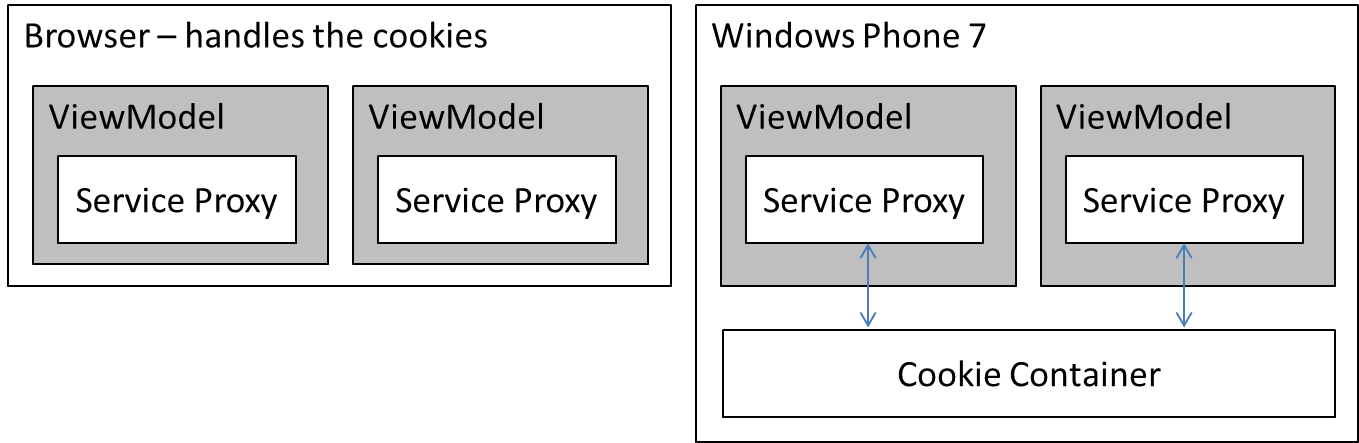
\includegraphics[width=14cm]{figures/cookies_situation}
\caption{Differences in cookies handling by Silverlight and Windows Phone 7 application}
\label{fig:cookies_situation}
\end{center}
\end{figure}

The initiation of the service in the Windows Phone 7 has to add to each service the same cookie container. This code cannot be part of the ViewModel, because than the ViewModel would not be reusable on Silverlight platform.

\begin{verbatim}
var service = new DataServiceClient();
service.CookieContainer = cookieContainer;
\end{verbatim}

For this reason the dependency injection pattern was extended to the client side. Static class \textit{ServicesFactory} contains an object implementing \textit{ICreator} interface. Different implementation of this interface can be provided depending on the situation.

\begin{verbatim}
public interface ICreator
{
    T GetObject<T>() where T : class;
}

public static class ServicesFactory
{
    public static ICreator Creator { get; set; }
    public static T GetObject<T>() where T: class {      
        return Creator.GetObject<T>();
    }
}
\end{verbatim}

The implementation of the \textit{ICreator}, which solves the problem of cookies container implements the \textit{GetObject<T>()} method using the fact that each implementation of the service has to also implement the \textit{ClientBase<T>} interface of the \textit{System.ServiceModel} namespace.

\begin{verbatim}
public Dictionary<Type, Type> services = new Dictionary<Type, Type>();

public void Register(Type iface, Type impl){
    services.Add(iface,impl);
}

public T GetObject<T>() where T : class
{
    var implem = services[typeof(T)];
    var instance = Activator.CreateInstance(implem);
    var client = instance as ClientBase<T>;
    var manager = client.InnerChannel.GetProperty<IHttpCookieContainerManager>();
    
    if (manager != null && manager.CookieContainer == null)
    {
        manager.CookieContainer = container;
    }
    
    return client as T;
}
\end{verbatim}
The implementation makes use of a dictionary of types which contains a type to be created for each interface. Before the use of the \textit{GetObject<T>()} method, this dictionary has to be filled with the interfaces and their implementations.
\begin{verbatim}
Register(typeof(DataService), typeof(DataServiceClient));
\end{verbatim}
In the ViewModel the instantiation of the WCF service is changed to the following declaration.

\begin{verbatim}
dataService = ServicesFactory.GetObject<DataService>();
\end{verbatim}
Different implementations of \textit{ICreator} can be then used for unit testing, such as an implementation which makes use of Rhino.Mock \footnote{Section \ref{tech:isolation} explains the use and choice of isolation frameworks used in this project} framework to predefine the behavior of the service.

\section{Building Model View ViewModel framework}
There exists a wide variety of MVVM frameworks, which makes the decision between them complicated. The features proposed by these frameworks are heterogeneous, but there is a set of basic functions which the MVVM framework should propose. I have identified these features and build own framework in order to achieve two aims:

\begin{itemize}
	\item Compose a framework which will contain only the features needed by the application.
	\item Compose two frameworks for Silverlight and Windows Phone 7, so that the ViewModels using these frameworks would not need any change in code and would compile for both platforms.
\end{itemize}

There are several features which can be proposed in a MVVM framework, however during the work on this thesis I have found three of them necessary.

\begin{itemize}
	\item  The possibility to create a command from lambda expressions.
	\item  The possibility to locate a ViewModel in the View which is outside of the scope defined by actual ViewModel.
	\item  The possibility to translate events into commands.
\end{itemize}

Several other features might be proposed or developed inside the MVVM framework such as tools for inter-ViewModel communication, dependency injection or background processing. However I did not found those necessary for the scope of the application.

\subsection{Creating commands from lambda expressions}
The foundation stone of MVVM pattern is the possibility of WPF or Silverlight to bind not only the properties but also the actions. Several components (such as Buttons, Panels and Lists) contain Dependency Properties\footnote{Dependency Property is a special type of a property which can be set through data binding} which expect to be bound to a property implementing \textit{ICommand} interface. This interface encapsulates an action which is executed when the command is invoked. 

This however means, that for each new command in the ViewModel a new class would have to be implemented, such as the following one:
\begin{verbatim}
public class SaveDataCommand : ICommand
{	
    public void Execute(object parameter)
    {
        DataService.SaveData(parameter as ViewModel);
    }
    
    public void CanExecute(object parameter)
    {
        parameter != null;
    }
}
\end{verbatim}

This would cause a lot of boiler plate code for every new command. Since it is only the content of \textit{Execute} and \textit{CanExecute} methods which changes for each command, generic implementation of the \textit{ICommand} interface can be invented.

\begin{verbatim}
public class GenericCommand<T> : ICommand
{
    private readonly Action<T> execute;
    private readonly Predicate<T> canExecute;
    
    public GenericCommand(Action<T> ex, Predicate<T> canEx = null){
       execute = ex;
       canExecute = caEx;
    }
    public bool CanExecute(object parameter)
    {
        return canExecute == null ? true : canExecute((T)parameter);
    }
    
    public void Execute(object parameter)
    {
        execute((T)parameter);
    }
}
\end{verbatim}
This generic class can greatly simplify the creation of new commands. In the ViewModel a new command can be defined using lambda expressions in one line of code.

\begin{verbatim}
public ICommand SaveDataCommand
{
    get { return new GenericCommand<UserData>(
       (x) => DataService.SaveData(x),
       (x) => x.Name != null);
    }
}
\end{verbatim}
This assignment defines the action which should be execute as \textit{DataService.SaveData(param)} and supposing that the \textit{UserData} object contains property \textit{Name} the action will get executed only if the \textit{Name} is not null.

\subsection{Binding to events}
Not all visual components expose Dependency Properties which could be bound to \textit{ICommand} interface. Several graphical components expose only events. Therefor there is a need for simple way to create a command from an event. The solution here is to implement a class based on \textit{TriggerAction<T>}. This class can be attached to an arbitrary event of a graphical user element of generic type T. By overriding the \textit{Invoke} the action can be defined which should be executed when event is fired.

\begin{verbatim}
public class EventToCommand : TriggerAction<FrameworkElement>
{
    //Command and Parameter have to be backed up by Dependency Properties
    //in order to enable binding
    public bool BindParameters {get;set;}
    public ICommand Command {get;set;}
    public object Parameter {get;set;}
    
    protected override void Invoke(object parameter)
    {
       if (parameter != null && BindParameters)
       {
          Parameter = parameter;
       }
       
       if (Command != null)
       {
          Command.Execute(CommandParameter);
       }
    }
}
\end{verbatim}
To use this class the \textit{Command} property has to be bound to a value in ViewModel. The Boolean value \textit{BindParameters} specifies if the parameter of the event should be passed directly as the parameter to the command. Any other object can be passed as the parameter by binding the \textit{Parameter} property.

The following snippet demonstrates the binding of "drop" event of a grid component.

\begin{verbatim}
<Grid>
	<i:Interaction.Triggers>
	    <i:EventTrigger EventName="Drop">
	        <mvvm:EventToCommand Command="{Binding Path=DropCommand}" ... />
	    </i:EventTrigger>
	</i:Interaction.Triggers>
</Grid>
\end{verbatim}

\subsection{Locating ViewModels}
When the \textit{DataContext} property of a particular View or User Control is set to certain ViewModel, then it is straightforward to bind TextBoxes, Labels or collections of this View to the values of selected ViewModel. The ViewModel "backs up" the View.

It turns complicated when there is a need to bind to values external to this ViewModel. Typical example of this situation is illustrated on figure \ref{fig:mvvm_locator} where a collection of items is show in a list. Each item contains a "remove" button which has to be bound to command defined in the parent ViewModel. Because each item in the list is bound to it's own ViewModel, the binding has to leave the \textit{DataContext} and bind to external (in this case parent) ViewModel.

\begin{figure}[h]
\begin{center}
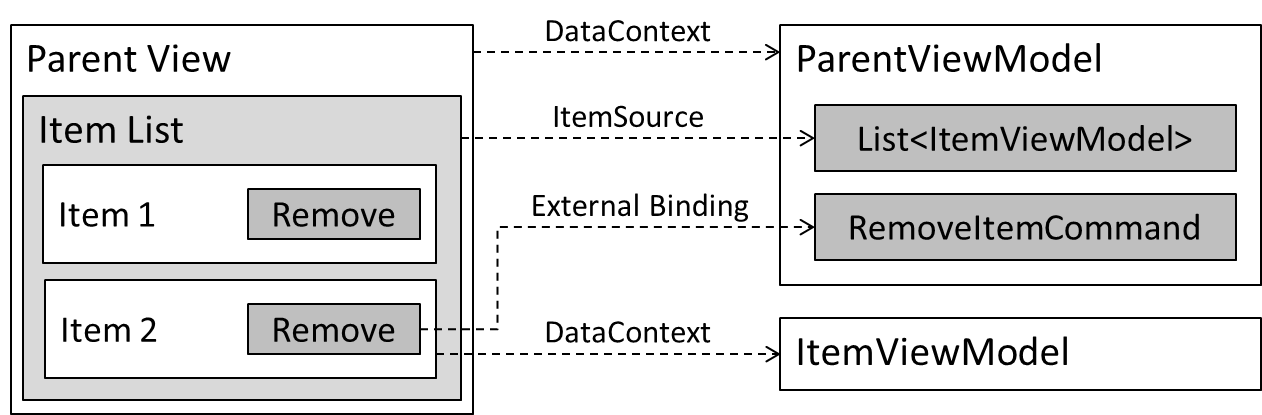
\includegraphics[width=14cm]{figures/mvvm_locator}
\caption{Binding to out of the scope ViewModel}
\label{fig:mvvm_locator}
\end{center}
\end{figure}

The solution to this issue is to create ViewModel locator class which is able to locate the ViewModel outside of the current \textit{DataContext} of current View and provide the properties of this ViewModel to the current View. One of the ways to implement this class is to create a component which can be placed to the XAML definition of the View and which will traverse the tree of graphic components and check the \textit{DataContext} of each component until it finds the demanded ViewModel.

\begin{verbatim}
public static object WalkUpTreeTillVM(this FrameworkElement obj, string vmName)
{
    var parent = obj;
    while (parent != null)
    {
        var context = parent.DataContext;

        if (context != null && context.GetType().Name == vmName)
        {
            return context;
        }

        parent = VisualTreeHelper.GetParent(parent) as FrameworkElement;
    }
    return null;
}
\end{verbatim}
In order to be able to use the result of the above stated method, \textit{ViewModelLocator} class is defined, which inherits from \textit{FrameworkElement} thus can be inserted directly into the XAML definition of the View.

\begin{verbatim}
public class ViewModelLocator : FrameworkElement
{
	public String ViewModelName {get;set;}
	
	//the Data property has to be backed up by Dependency Property to be bindable
	public object Data {get;set;}
	public DependencyProperty _data;

    protected void Loaded(object sender, RoutedEventArgs e)
    {
        if(ViewModelName != null)
        {
            //create binding between the component found by the traversing 
            //of the UI tree and the Data property
            Binding binding = new Binding();
            binding.Source = this.WalkUpTreeTillVM(ViewModelName);
            SetBinding(_data, binding);   
        }
    }
}
\end{verbatim}
Later this \textit{ViewModelLocator} can be used in the View, where the component which needs the data of particular ViewModel will bind to the exposed \textit{Data} property of this element.
\begin{verbatim}
<mvvm:ViewModelLocator x:Name="Parent" ViewModelName="ParentViewModel"/>

<ListBox ItemsSource="Items">
  <ListBox.ItemTemplate>
    <TextBlock Text={Binding Title}/>
    <!-- Command's binding is directed to the "ParentViewModel" -->
    <Button Command="{Binding Data.RemoveCommand,ElementName=Parent}"/>
  </ListBox.ItemTemplate>
</ListBox>
\end{verbatim}

\section {Implementation of Naive Bayes classifier}
Naive Bayes classifier has been implemented as new module to \textit{\href{machine.codeplex.com}{machine.codeplex.com}} library. The theoretical background is described in the section \ref{analysis:payment_categorization}. This section explains the implementation details.

The library \textit{machine.codeplex.com} contains two interfaces which define template for each new classifier: \textit{IModel} and \textit{IPredict}. The \textit{IModel} interface defines \textit{Generate} method which takes in the training data and creates an instance of \textit{IPredict}. The purpose of the model is the creation of the predictor, which in fact is ready to use classifier. \textit{IPredict} interface defines method \textit{T Predict(T item)} which assigns the category to given item.

Some additional methods are defined on both of these interface (such as serialization of the predictor to XML), but these methods are not important for banking application, therefor are not discussed.

The \textit{NaivaBayesModel} class converts all of the data in the learning set into matrix representation. Some of the internal structures of the \textit{machine.codeplex.com} library were changed to enable work with non-integer type categories.\footnote{Each transaction contains a property \textit{Tag} of the same type. Initially the \textit{machine.codeplex.com} library was not prepared to work with complex objects. Instead of that, categories of items had to be defined only using integer or double type values} In the process of converting to the matrix, a dictionary of tags is made and than only the integer index is used to reference each tag.

\subsection{Construction of the predictor}
The predictor needs four structures to hold important data in order to classify the item according to textual or continuous characteristics. These structures are one or two dimensional arrays. Each category or feature has assigned index (during the pre-processing) which enables the look-up in these arrays.

\begin{verbatim}
//Posteriori probability for each feature-category pair
//(where feature is binary property)
public double[ ][ ] Posteriori;

//A priori probability for each category
public double[ ] Apriori;

//Average value for each category-feature (where feature is continuous property)
public double[ ][ ] CategoryFeatureAvg;

//Variance for each category-feature (where feature is continuous property)
public double[ ][ ] CategoryFeatureVariance;
\end{verbatim}
The computation of a priori probability is the same for both type of features. 
\begin{verbatim}
Apriori[i] = CategoryCount[i] / TotalCount;
\end{verbatim}

The computation of a posteriori probability is done only for binary characteristics (containing the textual characteristics converted into binary characteristics).
For the binary features, the value at position [i,j] will be computed as follows.
\begin{verbatim}
Posteriori[i][j] = CategoryFeatureCount[j][i] / CategoryCount[i];
\end{verbatim}
Applied to the textual characteristics, this formula simply says that the probability of a text having category C with index (i) and containing word W (with index j) is the count of the items having the word W and category C divided by the total number of items having the category C.

For the continuous features, the posterioiri probability is estimated using the Gaussian distribution, using the average and variance values. The data arrays which contains average values and variances has to be filled before by the analysis of items in learning set. 

\begin{verbatim}
Normal(CategoryFeatureAvg[i][j],CategoryFeatureVariance[i][j],value)
\end{verbatim}

\subsection{Categorization process}
Once the arrays containing the a priori probability for each category and a conditional probability for each category-feature combination are prepared, the process of classification of an item consists of computing the probability of the item having the category for each category. The category with highest probability value will be selected.

To process the computation for one item and one category the classification has to loop over all features and multiply the probabilities.

\begin{verbatim}

foreach (var category in Categories)
{
  for (var feature in Features)
  {
      if(feature.IsContinuous){
      {
          var estimation = Normal( 
          			  CategoryFeatureAvg[category][j],
          			  CategoryFeatureVariance[category][j],
          			  value);
      }

      if (feature.Type.IsBinary))
      {
          var estimation = Posteriori[category][j];
      }
      probability = probability * estimation;
  }

  if (probability > maxProbability)
  {
      maxProbability = probability;
      maxCategory = category;
  }
}
item.SetValue(maxCategory);

\end{verbatim}
The process is composed of two loops, the type of each feature is determined (continuous or binary) and appropriated method is selected to get the value of the conditional probability. The classifier remembers the category which obtained the highest probability and the last statement categorizes the item.

\section {Using face recognition for easier authentication}
Face recognition is complicated machine learning task. The process of face recognition has two phases:

\begin{description}
	\item [Face detection] Face detection is the process of detecting the pixels in the image which represent the face. 
	\item [Face recognition] The actual task of recognizing the face by analyzing the part of the image identified during the face detection phase.
\end{description}

Face recognition brings in several problems which are completely unique to this domain and which make it one of the most challenging in the group of machine learning problems.

\begin{description}
	\item [Illumination problem] Due to the reflexivity of human skin, even a slight change in the illumination of the image can widely affect the results.
	\item [Pose changes] Any rotation of the head of a person will affect the performance.
	\item [Time delay] Due to the aging of the human individuals, the database has to be regularly updated.
\end{description}

\subsection{Eigenface-based face recognition}
There are several methods and algorithms which can be used to perform face recognition. Section \ref{tech:face_recognition} discusses the different methods. Eigenface algorithm was chosen because of the availability of several open source implementations and because of it's relative simplicity. Section \ref{tech:eigenface} describes the details of the algorithm.
The algorithm is based on Principal Component Analysis (PCA) and as such, follows the pattern applied by other statistical methods:

\begin{itemize}
	\item Compute the distance between the captured image and each of the images in the database.
	\item Select the example from the database, which is closest to the processed image (the one with the smallest distance to captured image). If the distance is not too big – label the image as concrete person. 	
\end{itemize}

The eigenfaces algorithm therefor has to define how to compute the distance between two images. To overcome this issue the PCA algorithm creates a set of principal components, which are called eigenfaces. Eigenfaces are images, that represent the main differences between all the images in the database.

The recognizer first finds an average face by computing the average for each pixel in the image. Each eigenface represents the differences from the average face. First eigenface represents the most significant differences between all images and the average image and the last one the least significant differences.

Figure \ref{fig:avarage_face} visualizes the average image created by analyzing the faces of 10 consultants working at OCTO Technology, having 5 images of each consultant. Figure \ref{fig:eigenfaces} shows the first five eigenfaces of the same dataset.

\begin{figure}[h]
\begin{center}

\includegraphics[width=3cm]{figures/avg}
\caption{Average face}
\label{fig:avarage_face}
\end{center}
\end{figure}

\begin{figure}[h]
\begin{center}
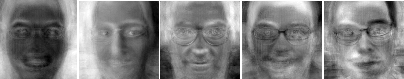
\includegraphics[width=10cm]{figures/eigenfaces}
\caption{First five eigenfaces created by analyzing images of 10 consultants working at OCTO Technology}
\label{fig:eigenfaces}
\end{center}
\end{figure}

After the creation of the eigenfaces, each image can be represented as a composition of these faces. Each image can be thus represented as a vector, where the elements of the vector are the coefficients given to each eigenface.

The distance between two images can be computed as the distance between two points in N-dimensional space, where N is the number of eigenfaces. For computing the distance, the Euclidean distance formula is used.

\subsection{Open Source libraries for Eigenfaces algorithm}
Eigenfaces based algorithm has already been developed in several languages and is available as part of existing image processing and machine learning libraries. To use eigenfaces in C\# EmguCV library can be used. EmguCV is a .NET wrapper for OpenCV library, written in C++ by Intel and published as open-source.\footnote{OpenCV library is released under BSD license and is free for academic and commercial use. It has been written in C++, with C and Python interfaces. EmguCV is written in C\# and uses the ability of .NET code to call methods from unmanaged assemblies.}

Using EmguCV means that any function inside OpenCV library can be called without the need of using constructs such as \textit{DLLImport} directive and without the need of knowing the exact structure of the OpenCV library.

The fact that EmguCV uses unmanaged DLL libraries, can pose problems for application interoperability. When compiled, .NET assemblies and programs are designed to run on every processor. If the the solution uses unmanaged libraries it is usually safe to include 32-bit assemblies, to assure the compatibility of the program on 32-bit machine.

However Azure cloud platform runs on 64-bit machines and furthermore it is not possible to load 32-bit library on this platform. Thus 64-bit versions of all external DLL libraries have to be used.

Including 64-bit assemblies can rise another issues also while developing and testing the software. The web server integrated in Visual Studio which is usually used for debugging (called Cassini) supports only 32-bit applications. Thus a local IIS server has to be created for debugging and testing.

\subsection{Process of face recognition}
The majority of the face recognition process is executed on the server side. Figure \ref{fig:face_recognition} depicts the phases in the training and face recognition processes.

\begin{figure}[h]
\begin{center}
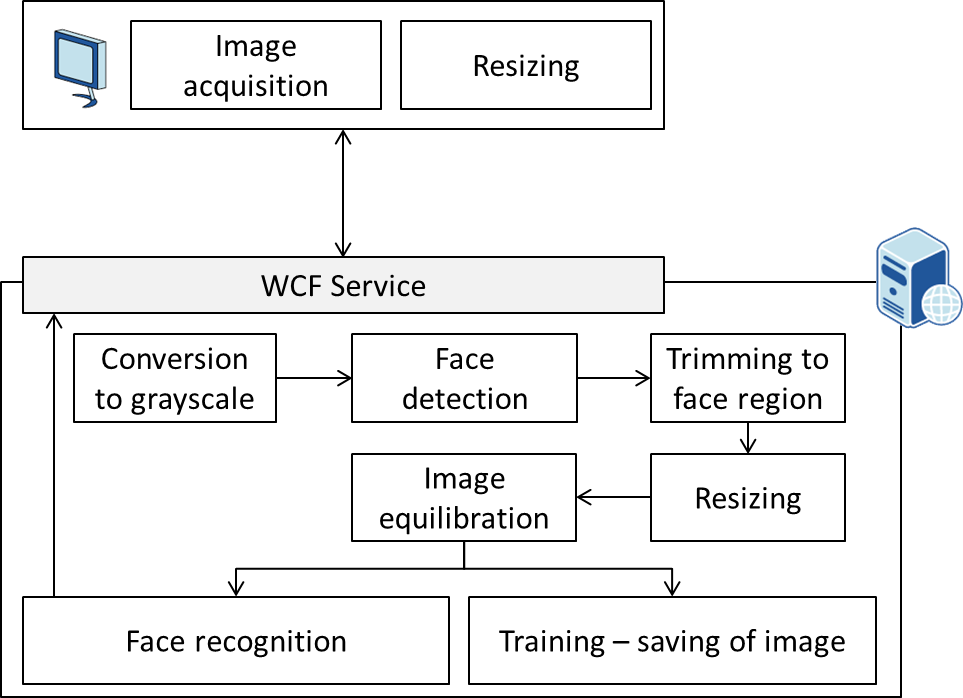
\includegraphics[width=14cm]{figures/face_recognition}
\caption{The process of face recognition}
\label{fig:face_recognition}
\end{center}
\end{figure}

\subsection{Capturing the image}
Since the version 4 Silverlight gives us the possibility to use the camera to capture images or videos using the \textit{CaptureSource} class. The following snippet shows how to access and start the camera.
\begin{verbatim}
var source = new CaptureSource();
source.VideoCaptureDevice = 
CaptureDeviceConfiguration.GetDefaultVideoCaptureDevice();
source.CaptureImageCompleted += 
new EventHandler<Args>(captureCompleted);

if (captureSource.State != CaptureState.Started)
{   
    if (CaptureDeviceConfiguration.RequestDeviceAccess())
        captureSource.Start();
}	
\end{verbatim}
To visualize the content of \textit{CaptureSource} the \textit{VideoBrush} can be used and applied to any graphical component (such as Rectangle or Ellipse).

\begin{verbatim}
var vidBrush = new VideoBrush();
vidBrush.Stretch = Stretch.Uniform;
vidBrush.SetSource(captureSource);
Rectangle.Fill = vidBrush;	
\end{verbatim}

Silverlight is asynchronous environment, where the user interface thread (UI thread) cannot be used by blocking operations. For that reason the developer has to set the callback for the \textit{CaptureImageCompleted} event. The following code is executed within the callback.

\begin{verbatim}
private void captureCompleted(Object sender, Args e)
{
    var image = e.Result;
    switch(appMode)
    {
        case AppMode.Recognition:
            client.RecognizeAsync(image.Pixels);
            break;
        case AppMode.Training:
            client.TrainFaceAsync(image.Pixels, label);
    }
}
\end{verbatim}

As a result of the capture, \textit{WritableBitmap} object is obtained, which has a \textit{Pixels} property of type \textit{int[]}. This property holds all the pixels of the image in one dimensional array created by aligning all the rows of the image to one array. Each pixel is represented as \textit{Integer}. Each color is thus represented using 32-bits.

This array has to be sent to the server. When the application is in training mode, also the label of the image is sent. If the application is in recognition mode, only the image is sent and the label of the image should be received.

\subsection{Server side recognition process}
Face recognition has two phases: face detection and face recognition. EmguCV can be used for both tasks. 

The first step which has to be taken is the detection of the face and clipping of the image. EmguCV uses \textit{Image<color type,depth>} structure for treating images, so the array of pixels has to be converted to this representation. Later the application uses the \textit{HaarCascade} class to perform the face detection. Section \ref{tech:haarcascade} contains additional information about Haar Cascade face detection.

\begin{verbatim}
var inBitmap = ConvertToBitmap(pixels, iSize);
var grayframe = new Image<Gray, byte>(inBitmap);
var haar = new HaarCascade(getHaarCascade());

var faces = haar.Detect(grayframe,
						  1.2,
						  3,
						  HAAR_DETECTION_TYPE.DO_CANNY_PRUNING,
						  new Size(30,30));
	
if (faces.Count() != 1)
    return null;

var face = faces[0];
var image = grayframe.Copy(face.rect);
\end{verbatim}

The image is converted to gray-scaled image where each pixel has 8 bits. Once the face is detected (and if there was only one face), the rectangle encapsulating the face is copied to a new image structure. Before passing the image to the recognition, we can reduce the noise created by different illumination situations by equalizing the image.

Histogram equalization is a technique to improve the contrast and adjust the brightness of the image. EmguCV gives us the possibility to call the equalize function which resides in OpenCV. Figure \ref{fig:image_equalization} visualizes the changes done by image equalization.

\begin{figure}[h]
\begin{center}

\includegraphics[width=8cm]{figures/equalization}
\caption{Image equalization}
\label{fig:image_equalization}
\end{center}
\end{figure}

For recognition task EmguCV contains \textit{EigenObjectRecognizer} class, which needs several arguments to be created:
\begin{description}
	\item [Images and labels] Array of images and corresponding array of labels.
	\item [Eigen Distance Threshold] Eigenfaces algorithm measures the distance between images. This thresholds defines the maximal distance needed to classify the image as concrete person. Big values such as 5000 will make the classifier to return the closest match, even if the probability that the person has been recognized is quite small. Values around 500 assures reasonable results.
	\item [MCvTermCriteria] \textit{McvTermCriteria} is a class which represents OpenCV structure for terminating iterative algorithms. It is composed of two numbers the first being the number of iterations and the second one is demanded accuracy. For some algorithm it makes sense to iterate until the accuracy is not bellow certain threshold. For eigenfaces algorithm it is the number of iterations which is important and it will impact the number of eigenfaces created.
\end{description}

The actual face recognition uses the method defined above to detect and trim the face. The resulting image is than passed to the recognizer. And the found label is passed through WCF service to the client application.

\begin{verbatim}
var termCrit = new MCvTermCriteria(40, accuracy);
var recognizer = 
	new EigenObjectRecognizer(trainedImages,labels,
             		eigenDistanceThreshold,ref termCrit);
             		
var imgFace = DetectAndTrimFace(pixels, size);
var label = recognizer.Recognize(imgFace);
\end{verbatim}

The face-detection phase is quite instantaneous. OpenCV already offers a set of HaarCascade features. The creation of these features is much more time consuming, than their usage.

If the database of faces does not change, the recognizer can be created only once and than can be shared every-time there is a request for recognition. This of course is not possible when the image database changes. In that case the recognizer has to be  recreated. There is no possibility to add new image to existing recognizer.

The bottleneck of this approach is still the network over which the image has to be passed from the client to the server. To minimize the data which has to be transferred, alternative approach could be used with face detection on the client side, which would lower the amount of pixels to be transferred to the server side. \footnote{There is an open-source project \href{facelight.codeplex.com}{facelight.codeplex.com} written for Silverlight which uses search for skin color regions and might be used to perform the face recognition on the client side.}.

\section {Implementation of Electronic vault}
Azure Blob Storage proposes two types of application interfaces. 

\begin{itemize}
	\item .NET Application interface
	\item HTTP REST Application interface
\end{itemize}

.NET API is a set of classes which can be used on the server side to access the storage. The following snippet shows, the process of uploading the file to Azure Blob Storage using only the server side interface.

\begin{verbatim}
var account = CloudStorageAccount.FromConfigurationSetting("connStr");
var client = account.CreateCloudBlobClient();

var container = client.GetContainerReference("container");
container.CreateIfNotExist();
var blob = container.GetBlobReference("fileName");
blob.UploadByteArray(data);
\end{verbatim}

The connection string which is used to connect to the storage contains the applications access key. This API runs only within the Azure environment. This means that application which would like to make this type of server side calls has to be deployed to the Azure platform.

REST API is completely platform independent and uses HTTP as its transport protocol to execute actions, upload and download data from the storage. The creation of the HTTP request depends on the platform of the client. In C\# we can use the following code:

\begin{verbatim}
public void UploadFile(Uri url){
  var request = (HttpWebRequest)ClientHttp.Create(url);
  request.Method = "PUT";
  request.Headers["x-ms-meta-comment"] = "my comment";
  request.Headers["x-ms-meta-author"] = "current user";
  request.BeginGetRequestStream(WriteData, webRequest);
}

private void WriteData(IAsyncResult result)
{
  var request = (HttpWebRequest)result.AsyncState;
  var stream = webRequest.EndGetRequestStream(result);       
  stream.BeginGetResponse(UploadFinish, webRequest);
}

private void UploadFinished(IAsyncResult result)
{
  if(result.IsCompleted){
    //Check the response
  }
}
\end{verbatim}

Note that the metadata of the file (comments, author) are added as headers to the HTTP Request.

In the proposed implementation it is advantageous to use both application interfaces. To give the Silverlight client direct access to the storage the REST API is used. This will also avoid passing of all the data through WCF Services and take significant data load of the servers. In case of generation of documents (such as transaction overviews), the documents will be generated and inserted to the vault using the server side API.

Is it has been explained in \ref{analysis:azureblob} Shared Access Signature mechanism is used to secure client side calls.
The generation of Shared Access Signature on the server side is simplified by the .NET API, which provides required methods. The following snippet illustrates the generation of Shared Access Signature, which will give the user read rights for the next 10 minutes.

\begin{verbatim}
var container = client.GetContainerReference("container1");
var permissions = new BlobContainerPermissions();
permissions.PublicAccess = BlobContainerPublicAccessType.Off;
container.SetPermissions(permissions);

var expDate = DateTime.UtcNow + TimeSpan.FromMinutes(10);
var sas = container.GetSharedAccessSignature(new SharedAccessPolicy()
{
   Permissions = SharedAccessPermissions.Read
});
\end{verbatim}

\subsection{Comparison with regular database}
The electronic vault could be also implemented using a SQL Server or Azure SQL (equivalent Cloud offer to SQL Server), by storing the files in the relational database. Here is a list of advantages which Azure Blob Storage has over relational database.

\begin{itemize}
	\item Blob Storage offers build-in support for the metadata for each file.
	\item Blob Storage has the ability of separating the files into blocks and thus provides better support for treatment of large files.
	\item The architecture of Blob Storage allows the access to each blob to be load-balanced and thus provides high access speed. However due to the dependence on network connection this is difficult to compare with SQL Server on premise or Azure SQL and no metrics have been published by Microsoft.
\end{itemize}